\begin{figure}[p]
  \centering
  \subfloat[Experiment 1]{\label{fig:rmse:e1}
\pgfplotsset{width=\textwidth,height=8cm}
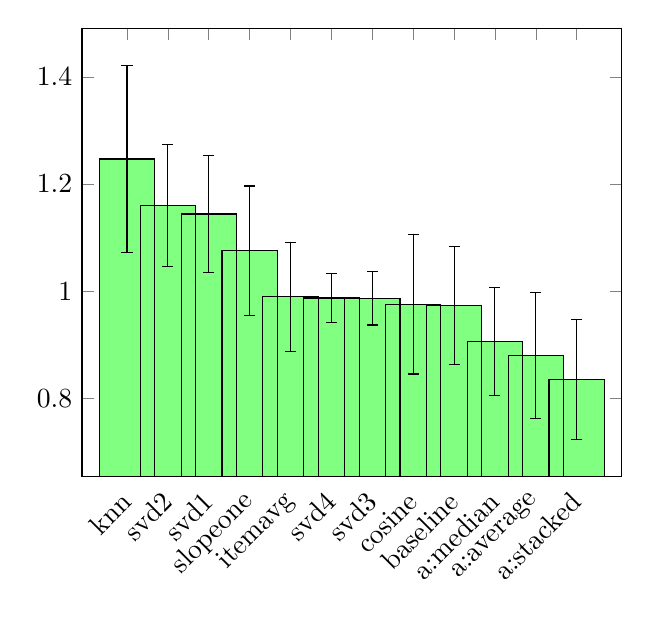
\begin{tikzpicture}
\begin{axis}[
      symbolic x coords={
        knn,svd2,svd1,slopeone,itemavg,svd4,svd3,cosine,baseline,a:median,a:average,a:stacked},
      xtick=data,
      x tick label style={rotate=45,anchor=east,yshift=-0.5em,xshift=-0.2em},
      bar width=20pt
    ]
    \addplot [ybar,fill=green!50,error bars/.cd,y dir=both,y explicit] coordinates {
      (knn, 1.2467) +- (0,0.17435) 
      (svd2, 1.1605) +- (0,0.11385)
      (svd1, 1.1441) +- (0,0.10985)
      (slopeone, 1.0756) +- (0,0.12075)
      (itemavg, 0.9895) +- (0,0.10115)
      (svd4, 0.9873) +- (0,0.0462)
      (svd3, 0.9865) +- (0,0.04955)
      (cosine, 0.9754) +- (0,0.12975)
      (baseline, 0.9738) +- (0,0.1098)
    %};
    %\addplot [ybar,fill=blue!50] coordinates {
      (a:median, 0.9065) +- (0,0.10025)
      (a:average, 0.8801) +- (0,0.1172)
      (a:stacked, 0.8352) +- (0,0.11125)
    };
\end{axis}
\end{tikzpicture}}

\vspace{1em}
 
  \subfloat[Experiment 2]{\label{fig:rmse:e2}
\pgfplotsset{width=\textwidth,height=8cm}
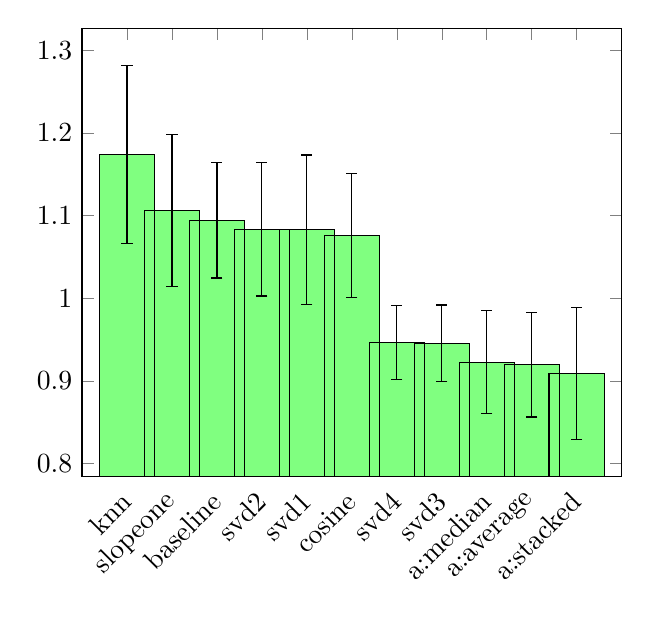
\begin{tikzpicture}
\begin{axis}[
      symbolic x coords={
        knn,slopeone,baseline,svd2,svd1,cosine,svd4,svd3,a:median,a:average,a:stacked},
      xtick=data,
      x tick label style={rotate=45,anchor=east,yshift=-0.5em,xshift=-0.2em},
      bar width=20pt
    ]
    \addplot [ybar,fill=green!50,error bars/.cd,y dir=both,y explicit] coordinates {
      (knn, 1.1740) +- (0,0.1077) 
      (slopeone, 1.1062) +- (0,0.0918)
      (baseline, 1.0945) +- (0,0.0700)
      (svd2, 1.0835) +- (0,0.0808)
      (svd1, 1.0829) +- (0,0.0905)
      (cosine, 1.0760) +- (0,0.0749)
      (svd4, 0.9467) +- (0,0.0446)
      (svd3, 0.9455) +- (0,0.0464)
    %};
    %\addplot [ybar,fill=blue!50] coordinates {
      (a:median, 0.9227) +- (0,0.0626)
      (a:average, 0.9193) +- (0,0.0630)
      (a:stacked, 0.9091) +- (0,0.0797)
    };
\end{axis}
\end{tikzpicture}}

\vspace{1em}

  \caption[Plots of Results for Experiments 1 \emph{\&} 2]{
    Plots of the average RMSEs for Experiments 1 \emph{\&} 2.
    The actual numbers are given in Tables \ref{table:results:e1}
    \emph{\&} \ref{table:results:e2}.
  }
  \label{plot:rmse}
\end{figure}


